\chapter[Referencial teórico]{Referencial teórico}

\section{Produtividade}

A produtividade é um conceito amplamente disseminado na teoria econômica. Segundo \citeonline{martins2005administraccao}, o conceito inicialmente foi apresentado em 1766 pelo economista fisiocrata francês François Quesnay.  Este termo pode ser definido como sendo a relação entre um  \textit{input} e um \textit{output} num determinado período de tempo, de tal forma que quanto maior for essa relação maior é a produtividade.

A produtividade de forma simples é definida como a relação entre a produção e os factores de produção utilizados. A produção é definida como os bens produzidos (quantidade de produtos produzidos). Os fatores de produção são definidos como máquinas, pessoas, matéria-prima entre outros. Quanto maior for a relação entre a quantidade produzida por fatores utilizados maior é a produtividade.

Podemos definir que a produtividade é a capacidade dos factores de produção para criar produto. A capacidade de associada à produtividade do trabalho, ou seja a quantidade de produto que se obtêm, utilizando uma unidade de trabalho. No entanto para o cálculo da produtividade temos de ter em mente não só a força trabalho, mas sim todos os fatores de produção associados.


\section{Eficácia}

A eficácia é uma medida definida para alcance dos resultados, segundo \citeonline{chiavenato1989recursos}. Pode ser descrita como o instrumento que mede a relação entre o efeito da ação, e os objetivos pretendidos.

A eficácia é a capacidade de produzir um efeito desejado, possível, planejado. Pode ser medida pela relação entre os resultados obtidos e os planejados; quer dizer, ser eficaz é conseguir atingir ou superar um dado objetivo ou propósito.

A relação entre a eficácia e a eficiência é complexa, porque é uma relação indireta. A eficácia é uma afirmação independente, enquanto a eficiência é uma condição, que nem sempre está atrelada à eficácia. Ou seja, eficiência tem a ver com dinamismo e rapidez e eficácia tem a ver com durabilidade e qualidade.

\section{Eficiência}

A Eficiência em contexto de produtividade é a capacidade de obter e conseguir produtos mais elevados em relação aos insumos necessários.

Habitualmente, a eficiência define-se como a capacidade (máquina, técnica, de uma pessoa ou empreendimento) de conseguir o melhor rendimento com menos utilização da capacidade produtiva, com o mínimo de erros, energia, tempo, dinheiro, mão-de-obra, materiais, máquinas ou, simplesmente, meios. Conforme afirma \citeonline{houaiss2001dicionario}.


Existem diversos tipos de eficiência, que se aplicam a áreas diferentes do conhecimento, eficiência ou rendimento refere-se à relação entre os resultados obtidos e os recursos empregados. É possível que o conceito de eficiência econômica ou global (EG) seja o mais amplo e pode ser subdividida, segundo \citeonline{farrell1957measurement}, em duas componentes: eficiência técnica global (ET) e eficiência alocativa (EA).

Eficiência técnica global (ET) envolve apenas os aspectos físicos do processo produtivo e indica a habilidade de uma organização na maximização da relação produto insumo.

A eficiência alocativa (EA) busca a melhor combinação dos insumos dentro das diferentes oportunidades de eficiência técnica global, de modo a minimizar custos. 

\section{Conjunto de Possibilidades de Produção}

Outro conceito relevante é as propriedades de tecnologia expressam as características do Conjunto de Possibilidades de Produção (CPP). Pode-se definir configuração de diferentes formatos para a fronteira empírica de produção e, portanto, a diferentes valores de eficiência para as unidades observadas. Estas propriedades estão associadas ao tipo de descarte permitido aos produtos e insumos e ao tipo de retorno de escala exibido pela tecnologia. Deste modo, para diferentes combinações de características de escala e descarte, temos diferentes tecnologias.

\citeonline{fare1994production} expressam as propriedades e descrevem as tecnologias bem como as medidas de eficiência relativa de acordo com o tipo de retorno e descarte assumido. Propõem, ainda, na ausência de melhores informações, o uso destas diferentes medidas para traçar o conjunto de possibilidades de produção e, com isto identificar e explorar as propriedades exibidas pela tecnologia.



\section{Análise Envoltória de dados}

A Análise Envoltória de Dados (DEA – sigla em inglês de \textit{Data Envelopment Analysis}) é uma ferramenta
não-paramétrica que avalia a eficiência técnica relativa de unidades produtivas, chamadas de Unidades
tomadoras de decisão (DMU, da sigla em inglês \textit{Decision Making Units}), comparando entidades que realizam tarefas similares e se diferenciam pela quantidade de recursos utilizados (\textit{inputs}) e de bens produzidos (\textit{outputs}). Segundo \citeonline{lins2000analise}, a história da Análise Envoltória de Dados começa com a dissertação para obtenção de grau de PhD de Edward Rhodes, sob a supervisão W. W. Cooper, publicada em 1978.

A publicação do modelo DEA-CCR por Abraham Charnes, William Cooper e Edward Rhodes (\citeyear{charnes1978measuring}), modelo desenvolvido por baseados nos trabalhos de \citeonline{debreu1951coefficient} e \citeonline{farrell1957measurement}, é reconhecida como o nascimento dos modelos de Análise de Envoltória de Dados (Data Envelopment Analysis), que permite determinar a eficiência de uma unidade produtiva comparativamente às demais, considerando-se os múltiplos insumos utilizados e os múltiplos produtos gerados \citeonline{gomes2008uso}.

DEA é uma ferramenta adequada tanto para avaliar a eficiência relativa das DMUs quanto para o estabelecimento de metas para DMUs consideradas ineficientes. As DMUs são comparadas de acordo com o conceito de eficiência de \citeonline{farrell1957measurement}, que consiste na razão entre a soma ponderada dos \textit{outputs} e a soma ponderada dos \textit{inputs} de cada DMU.

\subsection{DMU - \textit{Decision Making Units}}

Unidades tomadoras de decisão (Decision Making Units – DMUs) podem ser definidas como um conjunto de unidades a serem avaliadas. Essa avaliação deve ser homogênea, isto é, deve ter em comum a utilização dos mesmos \textit{inputs} e \textit{outputs}, realizar as mesmas ocupações, com os mesmos interesses, trabalhar nas mesmas condições de mercado e ter autonomia na tomada de decisões \citeonline{lins2000analise}.


As DMUs são comparadas de acordo com o conceito de eficiência de \citeonline{farrell1957measurement}, que consiste na razão entre a soma ponderada dos \textit{outputs} e a soma ponderada dos \textit{inputs} de cada DMU. 
Com a restrição de que todas as DMUs se encontrem na fronteira externa ou abaixo dela. Toda DMU observada que se encontre abaixo da fronteira de produção tem seu grau de ineficiência medido em relação a uma combinação de DMUs com melhores práticas e que compõem a faceta de fronteira mais próxima. A análise DEA gera como resultado:

\begin{itemize}
	\item Uma superfície envoltória que identifica as DMUs eficientes e ineficientes;
	\item Uma medida de eficiência métrica para cada DMU (à distância da fronteira, a fonte e o grau de ineficiência);
	\item Uma projeção da DMU sobre a fronteira;
	\item Um conjunto-referência (unidades específicas contra as quais uma DMU particular está sendo comparada).
\end{itemize}

\subsection{Análise Envoltória de dados - Modelos}



O método mais conhecido da abordagem de programação linear é a Análise por Envoltória
de Dados (\textit{Data Envelopment Analysis} – DEA), desenvolvido por \citeonline{charnes1978measuring}.


Em sua formulação matemática, considera-se que cada DMU $ k, k = 1, ..., n$, é uma unidade de produção que utiliza $r$ \textit{inputs} $x_{ik}, i =1, …, r$, para produzir $s$ \textit{outputs} $y_{jk}, j =1, …, s$. O modelo CCR, apresentado em (1), maximiza o quociente entre a combinação linear dos \textit{outputs} e a combinação linear dos \textit{inputs}, com a restrição de que, para qualquer DMU, esse quociente não pode ser maior que 1. Assim, para uma DMU o, $h_o$ é a eficiência; $x_{io}$ e $y_{jo}$ são os \textit{inputs} e \textit{outputs} da DMU o; $v_i$ e $u_j$ são os pesos calculados pelo modelo para \textit{inputs} e \textit{outputs}, respectivamente.

$$max\ h_0=\frac{\displaystyle\sum_{j=1}^{s} u_j y_{j0}}{\displaystyle\sum_{i=1}^{r} v_i x_{i0}} $$

$$sujeita\ a\; \frac{\displaystyle\sum_{j=1}^{s} u_j y_{jk}}{\displaystyle\sum_{i=1}^{r} v_i x_{ik}} \leq 1, k=1,...,n$$

$$u_j,v_i\geq0 \; \forall i, j$$
$$(1)$$

Mediante a transformação proposta por \citeonline{charnes1962programming}, esse modelo pode ser linearizado, transformando-se em um Problema de Programação Linear (PPL) apresentado em (2).

$$max\ h_0=\displaystyle\sum_{j=1}^{s} u_j y_{j0} $$

$$sujeita\ a\; \displaystyle\sum_{i=1}^{r} v_i x_{i0}=1$$

$$ \displaystyle\sum_{j=1}^{s} u_j y_{jk} - \displaystyle\sum_{i=1}^{r} v_i x_{ik}\leq 0, k=1,...,n$$



$$u_j,v_i\geq0 \; \forall i, j$$
$$(2)$$ 

DEA generaliza as medidas de \citeonline{farrell1957measurement} e busca medir a eficiência produtiva de unidades de produção com múltiplos insumos e múltiplos produtos. A abordagem DEA consiste na resolução de problemas de programação linear com o objetivo de projetar os produtores ineficientes tecnicamente até o conjunto de eficiência forte ou o conjunto de eficiência fraco.


Algumas das características que tornam a programação linear atrativa são:



\begin{itemize}
	\item Não requer dados sobre os preços para a construção da fronteira de produção empírica, bastando dados sobre as quantidades;
	\item A ineficiência técnica de unidades individuais se manifesta pela distância radial relativa à fronteira de produção (A fronteira de produção será, ou o conjunto de eficiência fraco ou o conjunto de eficiência forte);
	\item Por não ser paramétrica, é menos propensa a erros de especificação.
\end{itemize}


Há dois modelos DEA clássicos: o modelo CRS, também conhecido por CCR \citeonline{charnes1978measuring}, que considera retornos de escala constantes, e o modelo VRS, ou BCC \citeonline{banker1984some}, que considera retornos variáveis de escala e não assume proporcionalidade entre \textit{inputs} e \textit{outputs}.

O segundo, proposto por \citeonline{banker1984some}, o modelo BCC relaxa a imposição de tecnologia com retornos constantes de escala e admite que o conjunto de produção apresente retornos variáveis de escala. A tecnologia com retorno variável de escala assume o postulado de que todo plano de produção não observado que é uma combinação convexa dos planos de produção pertencentes ao conjunto de possibilidades de produção também
pertencem ao conjunto de possibilidades de produção. 


\section{Sugestão Para Conclusão}


A Análise Envoltória de Dados permite analisar a eficiência de unidades produtivas (DMUs) com múltiplos insumos (inputs) e múltiplos produtos (outputs) através da construção de uma fronteira de produção, também denominada de fronteira eficiente, linear por partes, de tal forma que as empresas que possuírem a melhor relação “produto/insumo” serão consideradas mais eficientes e estarão situadas sobre
esta fronteira e, as menos eficientes estarão situadas numa região inferior à fronteira, conhecida como envelope (envoltória).
A medida da eficiência de cada DMU é obtida através da divisão da soma ponderada dos insumos pela soma ponderada dos produtos, onde os pesos atribuídos às variáveis de entrada (Inputs) e de saída (Outputs) são calculados através de um problema de programação linear, que atribui às DMUs pesos que maximizem sua eficiência \citeonline{gomes2008uso}.

A Análise Envoltória de Dados pode ser considerada uma abordagem que mede excelência, uma vez que premia as DMU’s com as melhores práticas observadas. A classificação de uma unidade como eficiente ou ineficiente só depende do seu desempenho em transformar os inputs em outputs quando comparada com as outras unidades observadas \citeonline{gonzalez2003projeccoes}.




\section{Exemplo Figura}

\begin{figure}[h]
	\centering
	\label{fig01}
		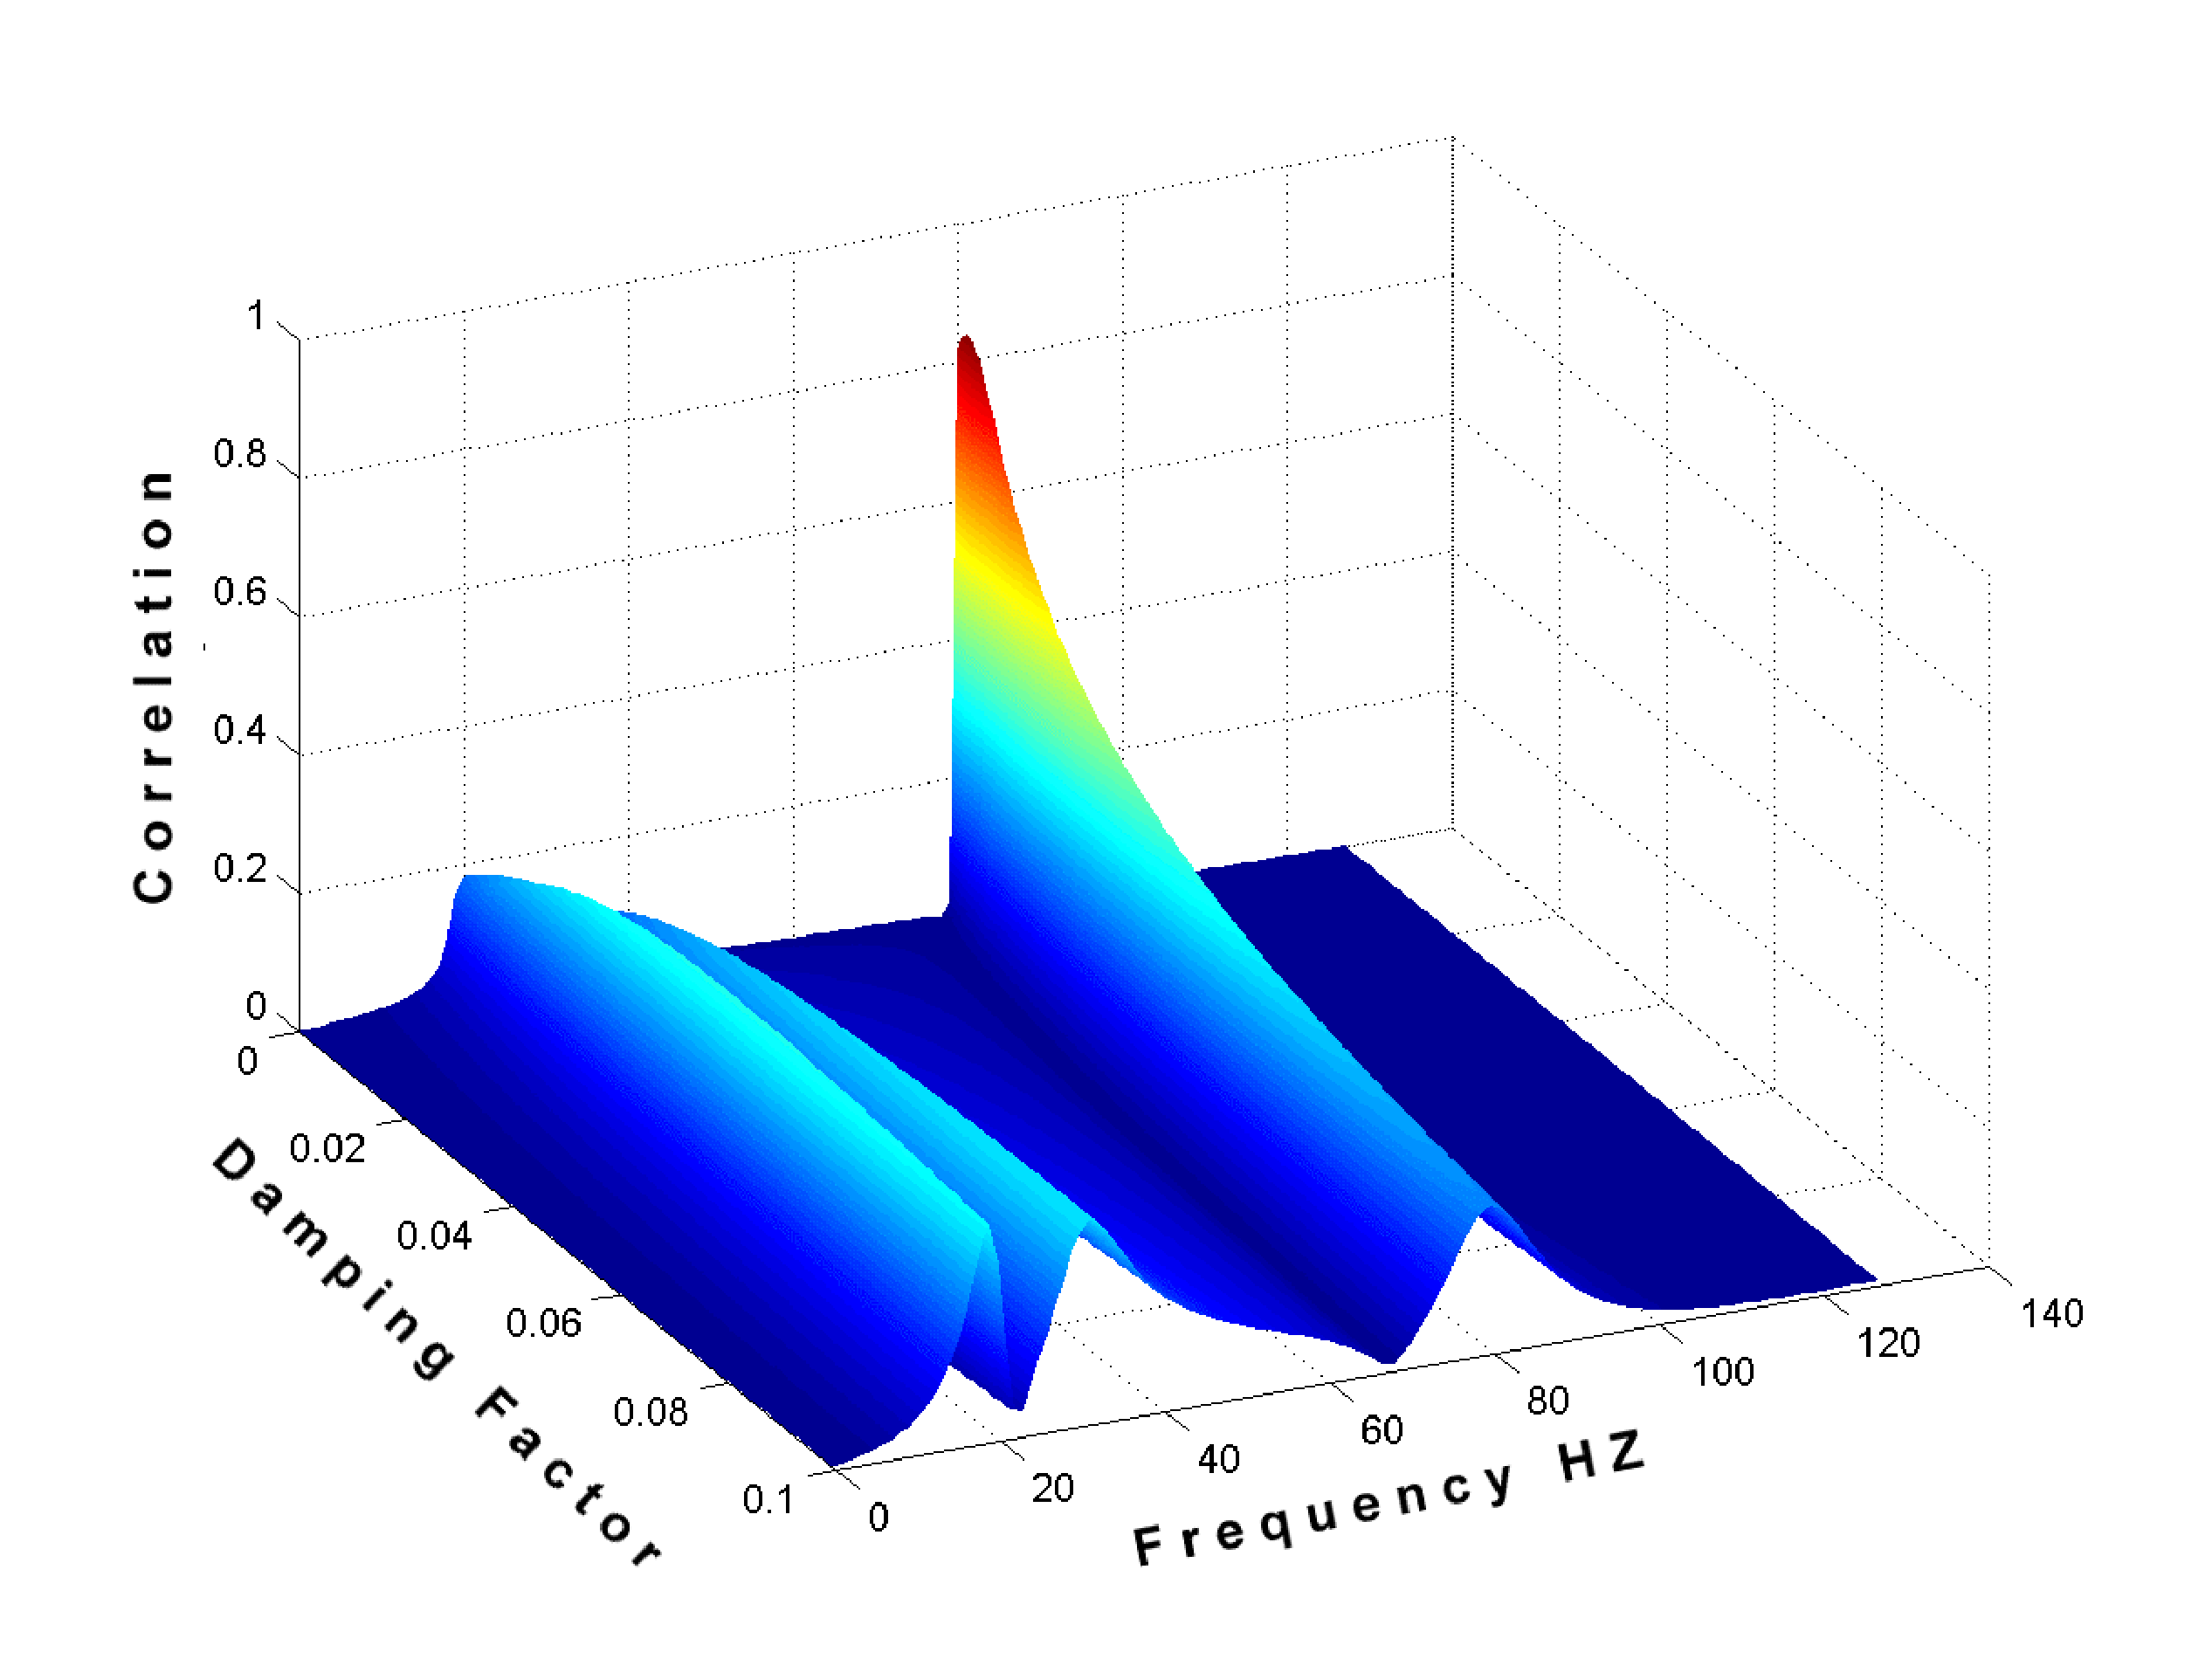
\includegraphics[keepaspectratio=true,scale=0.3]{figuras/fig01.eps}
	\caption{Wavelets correlation coefficients}
\end{figure}

\section{Exemplo Tabela}

\begin{table}[h]
	\centering
	\label{tab01}
	
	\begin{tabular}{ccc}
		\toprule
		\textbf{Processing type} & \textbf{Property 1} (\%) & 
		\textbf{Property 2} $[\mu m]$ \\
		\midrule
		Process 1 & 40.0 & 22.7 \\
		Process 2 & 48.4 & 13.9 \\
		Process 3 & 39.0 & 22.5 \\
		Process 4 & 45.3 & 28.5 \\
		\bottomrule
	\end{tabular}

	\caption{Propriedades obtidades após processamento}
\end{table}





